\section{Proof of the correctness lemma}\label{section:lemma_proof}
Let $T^{(p)} = \{T^{(p), A_i}\}$ be a constructed matrix $T$ by the algorithm in listing~\ref{lst:algo2} after $p-1$ loop iterations for $p \geq 2$, and $T^{(1)} = \{T^{(1), A_i}\}$ be a constructed matrix $T$ by this algorithm after initialization in lines 3-5. Note that the matrix $T$ returned by this algorithm is equal to $\sum_{p = 1}^{\infty} T^{(p)}$. Then the following lemma and theorem hold.

\begin{lemma}\label{lemma:correctness_appendix}
	Let $D = (V,E)$ be a graph, let $G =(N,\Sigma,P)$ be a grammar. Then for any $i, j$ and for any non-terminal $A \in N$, $index = T^{(p),A}_{i,j}$ and $index = (i,j,k,h,l) \neq \bot$ iff $(i,j) \in R_A$ and $i \pi j$, such that there is a derivation tree of the minimal height $h \leq p$ for the string $l(\pi)$  of length $l$ and a context-free grammar $G_A = (N,\Sigma,P,A)$.
\end{lemma}
\begin{proof}(Proof by Induction)
	
	\textbf{Base case}: Show that the lemma holds for $p = 1$. For any $i, j$ and for any non-terminal $A \in N$, $(i,j,k,h,l) = T^{(1), A}_{i,j}$ iff there is either $i \pi j$ of length $1$ that consists of a unique edge $e$ from the node $i$ to the node $j$ and $(A \rightarrow x) \in P$, where $x = l(\pi)$, or $i = j$ and $(A \rightarrow \varepsilon) \in P$, where $\varepsilon = l(\pi)$. Therefore $(i,j) \in R_A$ and there is a derivation tree of the minimal height $h = p = 1$, shown on Figure~\ref{tree1}, for the string $x$ and a context-free grammar $G_A = (N,\Sigma,P,A)$. Thus, it has been shown that the lemma holds for $p = 1$.
	
	\begin{figure}[h!]
		\centering
		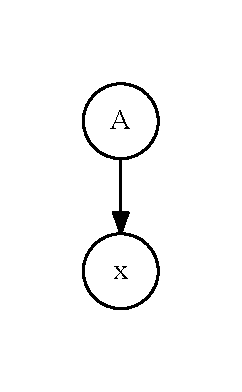
\includegraphics[width=2cm]{pictures/tree1.pdf}
		\caption{The derivation tree of the minimal height $p = 1$ for the string $x = l(\pi)$ where $x \in \Sigma \cup \{\varepsilon\}$.}
		\label{tree1}
	\end{figure}
	
	\textbf{Inductive step}: Assume that the lemma holds for any $p \leq (q - 1)$ and show that it also holds for $p = q$, where $q \geq 2$.
	
	The index $(i,j,k,h,l) = T^{(q),A}_{i,j}$ iff there is exists a rule $(A \to B C) \in P$ such that $(i,j,k,h,l) = M_{i,j}$ where $$M = T^{(q-1),A} + (T^{(q-1),B} \odot T^{(q-1),C}).$$ 
	
	Let $(i,j,k,h,l) = T^{(q-1),A}_{i,j}$. By the inductive hypothesis,\\ $(i,j,k,h,l) = T^{(q-1),A}_{i,j}$ iff $(i,j) \in R_A$ and there exists $i \pi j$, such that there is a derivation tree of the minimal height $h \leq (q-1)$ for the string $l(\pi)$ and a context-free grammar $G_A = (N,\Sigma,P,A)$. The statement of the lemma holds for $p = q$ since the height $h$ of this tree is also less than or equal to $q$.
	
	Now, let $(i,j,k,h,l) = (T^{(q-1),B} \odot T^{(q-1),C})_{i,j}$. By the definition of the binary operation $\odot$, $(i,j,k,h,l) = (T^{(q-1),B} \odot T^{(q-1),C})_{i,j}$ iff there are $r=k$, $(i,r,\_,h_1,l_1) = T^{(q-1),B}_{i,r}$ and $(r,j,\_,h_2,l_2) = T^{(q-1),C}_{r,j}$, such that $q = max(h_1, h_2) + 1$, $l = l_1 + l_2$. Hence, by the inductive hypothesis, there are $i \pi_1 r$ and $r \pi_2 j$, such that $(i,r) \in R_B$ and $(r,j) \in R_C$, and there are the derivation trees $T_B$ and $T_C$ of minimal heights $h_1 \leq (q-1)$ and $h_2 \leq (p-1)$ for the strings $w_1 = l(\pi_1)$, $w_2 = l(\pi_2)$ and the context-free grammars $G_B$, $G_C$ respectively. Thus, the concatenation of paths $\pi_1$ and $\pi_2$ is $i \pi j$, where $(i,j) \in R_A$ and there is a derivation tree of the minimal height $h = 1 + max(h_1, h_2)$, shown on Figure~\ref{tree2}, for the string $w = l(\pi)$ of length $l = l_1 + l_2$ and a grammar $G_A$.
	\begin{figure}[h!]
		\centering
		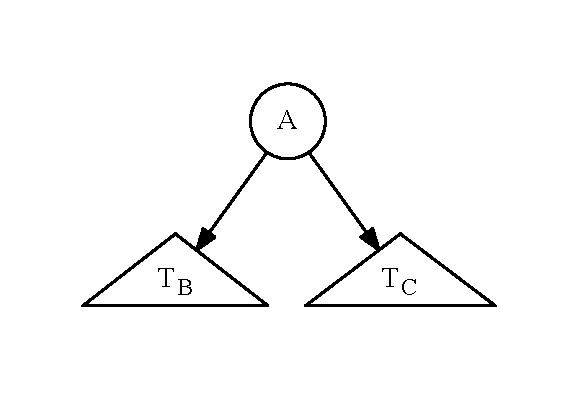
\includegraphics[width=5cm]{pictures/tree2.pdf}
		\caption{The derivation tree of the minimal height $h = 1 + max(h_1, h_2)$ for the string $w = l(\pi)$, where $T_B$ and $T_C$ are the derivation trees for strings $w_1$ and $w_2$ respectively.}
		\label{tree2}
	\end{figure}
	
	The statement of the lemma holds for $p = q$ since the minimal height $h = 1 + max(h_1, h_2) \leq q$. This completes the proof of the lemma.
\end{proof}

\begin{mytheorem}\label{thm:correct_appendix}
	Let $D = (V,E)$ be a graph and let $G =(N,\Sigma,P)$ be a grammar. Then for any $i, j$ and for any non-terminal $A \in N$, $index = T^A_{i,j}$ and $index = (i,j,k,h,l) \neq \bot$ iff $(i,j) \in R_A$ and $i \pi j$, such that there is a derivation tree of the minimal height $h$ for the string $l(\pi)$ of length $l$ and a context-free grammar $G_A = (N,\Sigma,P,A)$.
\end{mytheorem}
\begin{proof}
	
	Since the matrix $T = \sum_{p = 1}^{\infty} T^{(p)}$ for any $i, j$ and for any non-terminal $A \in N$, $index = T^A_{i,j}$ and $index = (i,j,k,h,l) \neq \bot$ iff there is $p \geq 1$, such that $index \in T^{(p),A}_{i,j}$. By the lemma~\ref{lemma:correctness_appendix}, $index = T^{(p),A}_{i,j}$ iff $(i,j) \in R_A$ and $i \pi j$, such that there is a derivation tree of the minimal height $h \leq p$ for the string $l(\pi)$  of length $l$ and a context-free grammar $G_A = (N,\Sigma,P,A)$. This completes the proof of the theorem.
\end{proof}

{\setlength{\tabcolsep}{0.4em}
	\begin{table*}[h]
		\caption{RDFs query $G_1$ (time is measured in seconds and memory is measured in megabytes)}
		\label{tbl:tableRDFQ1_appendix}
		\rowcolors{3}{}{lightgray}
		\begin{tabular}{| l | r  r | r  r | r  r | r  r | r  r |}
			\hline
			
			\multirow{3}{*}{Name}   &   \multicolumn{6}{|c|}{Relational semantics index}	&	\multicolumn{4}{|c|}{Single path semantics index} \\
			\cline{2-11}
			&	\multicolumn{2}{|c|}{RG\_CPU\textsubscript{rel}}	&	\multicolumn{2}{|c|}{RG\_CUSP\textsubscript{rel}}	&	\multicolumn{2}{|c|}{RG\_SPARSE\textsubscript{rel}} &	\multicolumn{2}{|c|}{RG\_CPU\textsubscript{path}}	&	\multicolumn{2}{|c|}{RG\_SPARSE\textsubscript{path}}	 \\
			\cline{2-11}
			&   Time & Mem &  Time     & Mem & Time     & Mem  &  Time     & Mem & Time     & Mem \\
			\hline
			\hline
			atom-primitive              & 0.016 & 1.2  & 0.016 & 0.1 & 0.005 & 0.1  & 0.033 & 1.5  & 0.008 & 0.1  \\
			biomedical-mesure-primitive & 0.016 & 0.6  & 0.012 & 0.1 & 0.005 & 0.1      & 0.027 & 1.3  & 0.007 & 0.1  \\
			core                        & 0.004 & 0.3  & 0.022 & 2.0   & 0.010  & 0.1      & 0.002 & 0.3  & 0.016 & 0.1  \\
			eclass\_514en                 & 0.067 & 13.8 & 0.075 & 14.0  & 0.166 & 16.0     & 0.195 & 31.2 & 0.496 & 26.0   \\
			enzyme                      & 0.018 & 5.9  & 0.021 & 0.1 & 0.018 & 4.0        & 0.029 & 8.1  & 0.043 & 6.0    \\
			foaf                        & 0.002 & 0.4  & 0.013 & 0.1 & 0.006 & 0.1      & 0.024 & 0.4  & 0.009 & 0.1  \\
			funding                     & 0.006 & 0.5  & 0.019 & 0.1 & 0.006 & 0.1      & 0.057 & 0.5  & 0.009 & 0.1  \\
			generations                 & 0.002 & 0.3  & 0.010  & 0.1 & 0.004 & 0.1      & 0.013 & 0.3  & 0.005 & 0.1  \\
			go-hierarchy                & 0.091 & 16.3 & 0.433 & 650.0 & 0.108 & 121.2    & 0.976 & 92.0   & 0.336 & 125.0  \\
			go                          & 0.604 & 28.8 & 0.590  & 70.0  & 0.365 & 30.2     & 1.286 & 75.7 & 0.739 & 45.4 \\
			pathways                    & 0.011 & 0.1  & 0.019 & 0.1 & 0.007 & 0.1      & 0.021 & 0.5  & 0.021 & 2.0    \\
			people\_pets                & 0.017 & 0.4  & 0.025 & 0.1 & 0.007 & 0.1      & 0.031 & 0.6  & 0.011 & 0.1  \\
			pizza                       & 0.030  & 1.8  & 0.021 & 4.0   & 0.006 & 0.1      & 0.075 & 5.5  & 0.009 & 0.1  \\
			skos                        & 0.001 & 0.1  & 0.008 & 0.1 & 0.004 & 0.1      & 0.005 & 0.3  & 0.006 & 0.1  \\
			travel                      & 0.004 & 0.3  & 0.022 & 2.0   & 0.007 & 0.1      & 0.008 & 0.3  & 0.010  & 0.1  \\
			univ-bench                  & 0.002 & 0.3  & 0.010  & 0.1 & 0.005 & 0.1      & 0.013 & 0.3  & 0.007 & 0.1  \\
			wine                        & 0.017 & 3.5  & 0.032 & 6.0   & 0.009 & 0.1      & 0.117 & 7.1  & 0.015 & 0.2  \\
			\hline
		\end{tabular}
	\end{table*}
}



\section{Dataset description}\label{section:dataset}



In our evaluation we use dataset which contains the following parts.

{\setlength{\tabcolsep}{0.4em}
	\begin{table*}[h]
		\caption{RDFs query $G_2$ (time is measured in seconds and memory is measured in megabytes)}
		\label{tbl:tableRDFQ2}
		\rowcolors{3}{}{lightgray}
		\begin{tabular}{| l | r  r | r  r | r  r | r  r | r  r |}
			\hline
			
			\multirow{3}{*}{Name}   &   \multicolumn{6}{|c|}{Relational semantics index}	&	\multicolumn{4}{|c|}{Single path semantics index} \\
			\cline{2-11}
			&	\multicolumn{2}{|c|}{RG\_CPU\textsubscript{rel}}	&	\multicolumn{2}{|c|}{RG\_CUSP\textsubscript{rel}}	&	\multicolumn{2}{|c|}{RG\_SPARSE\textsubscript{rel}} &	\multicolumn{2}{|c|}{RG\_CPU\textsubscript{path}}	&	\multicolumn{2}{|c|}{RG\_SPARSE\textsubscript{path}}	 \\
			\cline{2-11}
			&   Time & Mem &  Time     & Mem & Time     & Mem  &  Time     & Mem & Time     & Mem \\
			\hline
			\hline
			atom-primitive          & 0.001 & 0.3  & 0.001 & 0.1 & 0.002 & 0.1   & 0.001 & 0.3  & 0.002 & 0.1   \\
			biomedical-mesure-primitive & 0.002 & 0.1  & 0.014 & 2.0   & 0.009 & 0.1   & 0.006 & 0.1  & 0.012 & 0.1   \\
			core                        & 0.001 & 0.3  & 0.006 & 0.1 & 0.004 & 0.1   & 0.003 & 0.3  & 0.005 & 0.1   \\
			eclass\_514en               & 0.035 & 6.5  & 0.020 & 16.0  & 0.100   & 12.0    & 0.123 & 17.7 & 0.127 & 18.0    \\
			enzyme                      & 0.006 & 3.9  & 0.006 & 0.6 & 0.010  & 0.1   & 0.012 & 5.3  & 0.008 & 0.4   \\
			foaf                        & 0.001 & 0.1  & 0.004 & 0.1 & 0.002 & 0.1   & 0.001 & 0.1  & 0.003 & 0.1   \\
			funding                     & 0.002 & 0.1  & 0.015 & 0.4 & 0.007 & 0.1   & 0.009 & 0.1  & 0.008 & 0.1   \\
			generations                 & 0.001 & 0.1  & 0.001 & 0.1 & 0.001 & 0.1   & 0.001 & 0.1  & 0.001 & 0.1   \\
			go-hierarchy                & 0.095 & 17.8 & 0.253 & 528.0 & 0.175 & 130.4 & 0.884 & 88.8 & 0.306 & 138.8 \\
			go                          & 0.306 & 25.8 & 0.240 & 84.0  & 0.181 & 25.4  & 0.918 & 78.1 & 0.219 & 34.2  \\
			pathways                    & 0.005 & 0.2  & 0.005 & 0.4 & 0.004 & 0.1   & 0.017 & 0.5  & 0.003 & 0.1   \\
			people\_pets                & 0.001 & 0.1  & 0.007 & 0.1 & 0.004 & 0.1   & 0.001 & 0.1  & 0.005 & 0.1   \\
			pizza                       & 0.002 & 0.3  & 0.012 & 0.2 & 0.008 & 0.1   & 0.010  & 0.3  & 0.009 & 0.1   \\
			skos                        & 0.001 & 0.1  & 0.001 & 0.1 & 0.001 & 0.1   & 0.001 & 0.1  & 0.002 & 0.1   \\
			travel                      & 0.001 & 0.1  & 0.007 & 0.1 & 0.005 & 0.1   & 0.001 & 0.1  & 0.005 & 0.1   \\
			univ-bench                  & 0.001 & 0.1  & 0.007 & 0.1 & 0.005 & 0.1   & 0.001 & 0.1  & 0.005 & 0.1   \\
			wine                        & 0.001 & 0.3  & 0.006 & 0.1 & 0.004 & 0.1   & 0.002 & 0.3  & 0.004 & 0.1  \\
			\hline
		\end{tabular}
	\end{table*}
}

{\small
	\setlength{\tabcolsep}{0.4em}
	\begin{table}[h]
		\caption{RDFs properties}
		\label{tbl:propRDF}
		\rowcolors{2}{}{lightgray}
		\begin{tabular}{| l | c | c | c | c |}
			\hline
			Name                  & \#V    & \#E     & \#type &\#subClassOf \\
			\hline
			\hline
			atom-primitive				& 291		& 685		& 138	& 122	\\
			univ-bench					& 179		& 413		& 84		& 36		\\
			travel						& 131		& 397		& 90		& 30		\\
			skos							& 144		& 323		& 70		& 1		\\
			people\_pets					& 337		& 834		& 161	& 33		\\
			generations					& 129		& 351		& 78		& 0		\\
			foaf							& 256		& 815		& 174	& 10		\\
			biomed-mesure-prim   	    & 341		& 711		& 130	& 122	\\
			funding						& 778		& 1480		& 304	& 90               \\
			pizza						& 671		& 2604		& 365	& 259              \\
			wine							& 733		& 2450		& 485	& 126              \\
			core							& 1323		& 8684		& 1412	& 178              \\
			pathways						& 6238		& 37196		& 3118 	& 3117             \\
			go-hierarchy					& 45007		& 1960436	& 0		& 490109           \\
			enzyme						& 48815		& 219390		& 14989	& 8163             \\
			eclass\_514en				& 239111		& 1047454	& 72517	& 90962            \\
			go							& 272770		& 1068622	& 58483	& 90512            \\
			\hline
		\end{tabular}
	\end{table}
}



\begin{itemize}
\item The real-world data RDFs provided in CFPQ\_Data dataset\footnote{CFPQ\_Data dataset GitHub repository: \url{https://github.com/JetBrains-Research/CFPQ_Data}. Access date: 12.11.2019.} from~\cite{Mishin:2019:ECP:3327964.3328503}.
\item Geospecies (RDF which contains information about biological hierrarchy\footnote{The Geospecies RDF: \url{https://old.datahub.io/dataset/geospecies}. Access date: 12.11.2019.} and same-generation query over \textit{broaderTransitive} relation) is provided in~\cite{Kuijpers:2019:ESC:3335783.3335791} and integrated in our evaluation with CFPQ\_Data.
\item It was shown in~\cite{Mishin:2019:ECP:3327964.3328503} that matrix-based algorithm is performant enough to handle bigger RDFs than those used in the initial datasets, such as~\cite{RDF}.
So, we add several big RDFs to CFPQ\_Data and use them in our evaluation.
New RDFs: \textit{go-hierarchy, go, enzime, core, pathways} are from UniProt database\footnote{Protein sequences data base: \url{https://www.uniprot.org/}. RDFs with data are avalable here: \url{ftp://ftp.uniprot.org/pub/databases/uniprot/current_release/rdf}. Access date: 12.11.2019}, and \textit{eclass-514en} is from eClassOWL project\footnote{eClassOWL project: \url{http://www.heppnetz.de/projects/eclassowl/}. eclass-514en file is available here: \url{http://www.ebusiness-unibw.org/ontologies/eclass/5.1.4/eclass_514en.owl}. Access date: 12.11.2019.}.
\end{itemize}

The properties of the RDFs from the dataset are given in table \ref{tbl:propRDF}. 
Geospecies RDF contains 450609 vertices, 2311461 edges, and 20867 edges labeled by \textit{broaderTransitive}.
Note that while the number of edges labeled by \textit{broaderTransitive} is equal to provided in~\cite{Kuijpers:2019:ESC:3335783.3335791}, the total number of vertices and edges is bigger. It is because we naively convert each triple from RDF to edge in the graph, while J. Kuijpers et al. use special \textit{neosemantics}\footnote{Neosemantix is an RDF processing plugin for Neo4j. Web page: \url{https://neo4j.com/labs/nsmtx-rdf/}. Access date: 30.03.2020.} plugin which can, for example, handling multivalued properties accurately.  

The variants of the \textit{same-generation query}~\cite{FndDB} are used in almost all cases because it is an important example of real-world queries that are context-free but not regular.
So, variations of the same generation query are used in our evaluation.
All queries are added to the CFPQ\_Data dataset.

We use two queries over \textit{subClassOf} and \textit{type} relations.
The first query is the grammar $G_1$:
\[
 \begin{array}{lcl}
   s  \rightarrow \textit{subClassOf}^{\ -1} \ s \ \textit{subClassOf}   & \quad & s  \rightarrow \textit{type}^{\ -1} \ s \ \textit{type}     \\
   s  \rightarrow \textit{subClassOf}^{\ -1} \ \textit{subClassOf}       & \quad & s  \rightarrow  \textit{type}^{\ -1}  \ \textit{type}

 \end{array}
 \]
The second one is the grammar $G_2$: \[s \rightarrow \textit{subClassOf}^{\ -1} \ s \ \textit{subClassOf} \mid \textit{subClassOf}\]

For geospecies we use same-generation query \textit{geo} from the original paper~\cite{Kuijpers:2019:ESC:3335783.3335791}: \[s \rightarrow \textit{broaderTransitive} \ s \ \textit{broaderTransitive}^{\ -1} \]
\[s \rightarrow \textit{broaderTransitive}  \ \textit{broaderTransitive}^{\ -1} \]


\section{Evaluation Details}\label{section:evaluation_appendix}

Results for RDFs querying with $G_1$ grammar are presented in table~\ref{tbl:tableRDFQ1_appendix}. Results for RDFs querying with $G_2$ grammar are presented in table~\ref{tbl:tableRDFQ2}.
We can see, that for small graphs time for both relational and single-path querying are similar for CPU and GPGPU versions, but for bigger graphs (\textit{go} and \textit{go-hierarchy}, for example) GPUPU version is more performant than CPU one.

\balance

